\section{Efficiently updatable neural networks}

NNUE (\reflectbox{NNUE} Efficiently updatable neural network) is a neural network architecture that allows for very fast subsequent evaluations for minimal input changes. It was invented for Shogi by Yu Nasu in 2018 \cite{nnue:2018}, later adapted to Chess for use in Stockfish in 2019 and may be used in other board games as well. Most of the information described in this chapter can be found in the excellent Stockfish documentation \cite{nnue-pytorch}.


...

goes very well with incremental updates

It is important to combine this with aggresive quantization techniques.


\begin{figure}[h]
\centering
\subfloat[\centering Linear layer]{{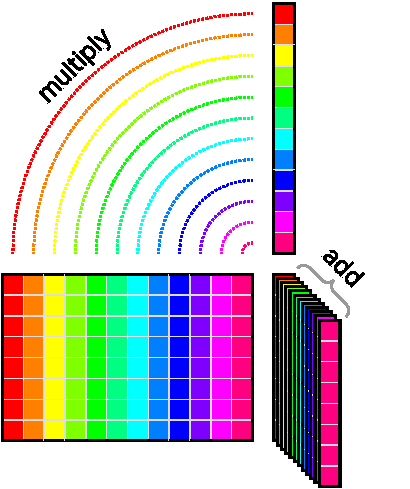
\includegraphics[width=5cm]{../assets/nnue/mv.pdf} }}%
\qquad
\subfloat[\centering Linear layer with sparse inputs]{{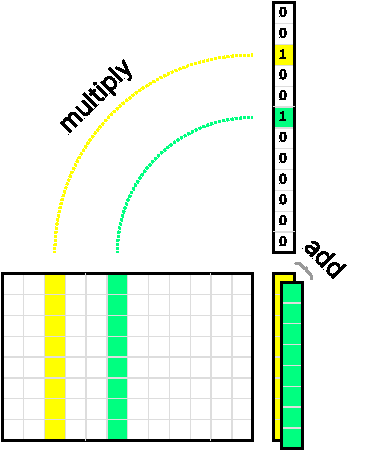
\includegraphics[width=5cm]{../assets/nnue/mvs.pdf} }}%
\caption{Linear layer operation comparison. Figures from \cite{nnue-pytorch}.}
\label{fig:linear_comparison}
\end{figure}



\subsection{Architecture}


arquitectura half, dos capas
for this thesis...


\subsection{Efficient updates}

pesada al principio y liviana al final, acumular filas de la primera capa en domove, undomove

\subsection{Stockfish quantization scheme}



This is text bla bla. \footnote[2]{This is a example footnote}



\textbf{Rango de activación}: en el modelo original usamos ClippedReLU, asi que queremos que el rango vaya de 0..1 a 0..127.


Siendo $\bm{x}$, $\bm{w}$ y $\bm{b}$ los parámetros de una capa lineal sin cuantizar e $\bm{y}$ la salida de la misma, se tiene que:

\begin{equation}
\begin{aligned}
\bm{y} &= \bm{x} \bm{w} + \bm{b} \\
s_a s_w \bm{y} &= (s_a \bm{x}) (s_w \bm{w}) + s_a s_w \bm{b} \\
\end{aligned}
\end{equation}



\vspace{1cm}
$s_o ((s_a \bm{x}) (s_w \bm{w}) + s_a s_w \bm{b}) = s_a s_w s_o \bm{y}$



\subsection{Network sparsity}

o combinar con 3.2?
poner graficos con la sparsity de cada feature set, decir que es muy esparso todo y que se podría mejorar aún más
